\chapter{Introduction\label{cha:intro}}
\epigraph{Learning is not a product of schooling, but the lifelong attempt to
acquire it}{\textit{Albert Einstein}}
\noindent
The concept of lifelong learning has become very popular over the last decade.
The original idea has gone through a lot of changes, through the stages of
continuing, recurrent, and adult education (Jarvis, 2004, pp. 46-55). On one
hand, the lifelong learning concept has an entirely economic background, where
the learners themselves are seen as tools for economic development and their
needs are firmly tied to the needs of the industry (Carter, 2008, pp. 112-114).
On the other hand, as stated by UNESCO, \LLLs is a
cultural policy which influences society and promotes changes (Boshier, 2000, pp. 12-
14). However, no matter which point of view is adopted, world economics, employment
policy and society are changing. The importance of lifelong learning is increasing. For
full participation in education, workplace, and society individuals today require well-
developed lifelong learning skills, developed from the early stages of their lives (Otala,
1997).

In addition to being a subject for political and economical discussions (Bagnall, 2009),
lifelong learning has been also established as a topic of interest in higher education, in
particular universities (Knapper and Cropley, 2000). Universities provide the
necessary organizational framework, theoretical principles and practical experience for lifelong
learning (Knapper and Cropley, 2000). This can be seen in the role and influence
of the universities in the educational systems of most countries as the “keepers of the
intellectual traditions of a nation” (Longworth, 2003, p. 96). Based on this background of
the importance of lifelong learning and the central role of universities, this PhD research
is focused on and explores the need for lifelong learning support in
universities. Chapter 2 is focused on discussing the background of lifelong learning. Its connection to universities, the current situation in this area and the problems associated with lifelong
learning in universities are shown in this chapter. 


\section{Reseach Goals}

\section{Research Design}

\section{Scope and Limitations}

\section{Thesis Structure and Outline}

\begin{figure}[htb]
\centering
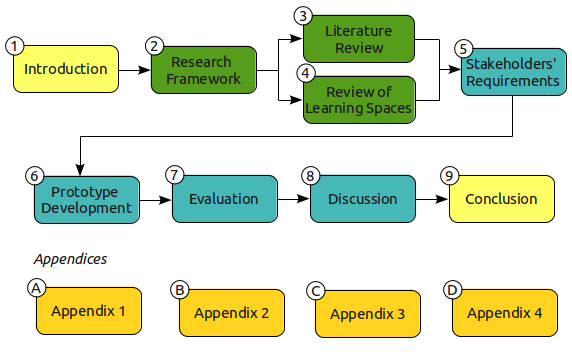
\includegraphics[width=0.8\textwidth]{CH1-F1-Thesis}
\caption{Thesis structure}
\label{fig:ts}
\end{figure}
